\documentclass{standalone}
\usepackage{tikz,pgfplots,calc}
\usetikzlibrary{positioning,calc}
\usetikzlibrary{arrows}
\usepackage{tkz-euclide}
\usetkzobj{all}

\tikzset{
  mynode/.style = {align = center}}

\usetikzlibrary{patterns}
\begin{document}
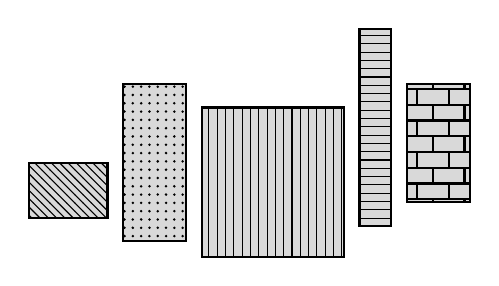
\begin{tikzpicture}[>=stealth', thick]
\draw [draw,  pattern=north west lines, pattern color = black, preaction={fill, gray!30}] (0, 0.3) rectangle (1, 1);
\draw [draw,  pattern = dots, pattern color = black, preaction={fill, gray!30}] (1.2, 0) rectangle (2, 2);
\draw [draw,  pattern = vertical lines, pattern color = black, preaction={fill, gray!30}] (2.2, -.2) rectangle (4, 1.7);
\draw [draw,  pattern = horizontal lines, pattern color = black, preaction={fill, gray!30}] (4.2, .2) rectangle (4.6, 2.7);
\draw [draw,  pattern = bricks, pattern color = black, preaction={fill, gray!30}] (4.8, .5) rectangle (5.6, 2.);
\end{tikzpicture}
\end{document}